\chapter{Introduction}
\label{cha:introduction}

In contemporary science and engineering applications, the volume of available data  is growing at an enormous rate. The emergence of this trend is  due to recent technological advances that have enabled the collection, transmission, storage and processing of data from every corner of our life, in the forms of images, videos, network traffic, email logs, electronic health records, genomic and genetic measurements, high-frequency financial trades, grocery transactions, online exchanges, and so on.
In the meantime, modern applications often require reasonings about an unprecedented scale of features or parameters of interest.
This gives rise to the pressing demand of developing {\em low-complexity} algorithms that can effectively distill actionable insights from large-scale and high-dimensional data. In addition to the curse of dimensionality, the challenge is further compounded when the data in hand are  noisy, messy, and contain missing features.



Towards addressing the above challenges, \emph{spectral methods} have emerged as a simple yet surprisingly effective approach to information extraction from massive and noisy data. In a nutshell, spectral methods refer to a collection of algorithms built upon the eigenvectors (resp.~singular vectors) and eigenvalues (resp.~singular values) of some properly designed  matrices generated from data. Remarkably, spectral methods lend themselves to a diverse array of applications in practice, including community detection in networks \citep{newman2006finding,abbe2017community,rohe2011spectral,mcsherry2001spectral}, angular synchronization in cryo-EM \citep{singer2011three,singer2011angular}, joint image alignment \citep{chen2016projected}, clustering \citep{von2007tutorial,ng2002spectral}, ranking \citep{negahban2016rank,chen2015spectral,chen2017spectral}, dimensionality reduction \citep{belkin2003laplacian}, low-rank matrix estimation \citep{achlioptas2007fast, keshavan2010matrix}, tensor estimation \citep{montanari2016spectral,cai2019tensor},  covariance and precision matrix estimation \citep{fan2013large,fan2020robust}, shape reconstruction \citep{li2004fast}, econometric and financial modeling \citep{fan2021recent}, among others.
Motivated by their applicability to numerous real-world problems, this monograph seeks to offer a unified and comprehensive treatment towards establishing the theoretical underpinnings for spectral methods, particularly through a statistical lens.






\section{Motivating applications}
\label{sec:motivating_examples}

At the heart of spectral methods is the idea that the eigenvectors or singular vectors of certain data matrices reveal crucial information pertaining to the targets of interest.
We single out a few examples that epitomize this idea.






\paragraph{Clustering.}


%
\begin{figure}
	\begin{center}
		\begin{tabular}{ccc}
			
\includegraphics[width=0.25\textwidth]{figures/adjacency_mean.png} & 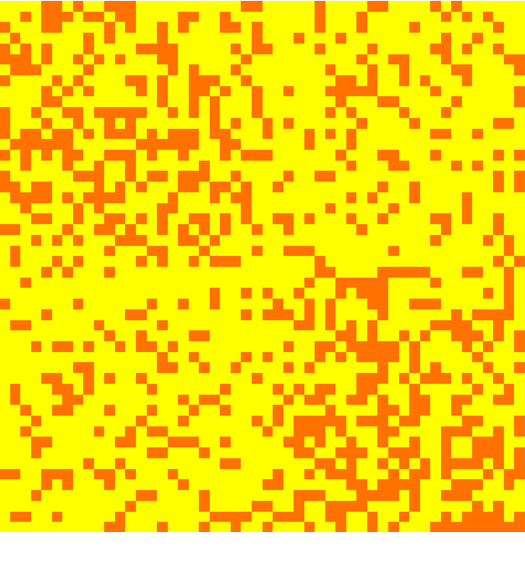
\includegraphics[width=0.25\textwidth]{figures/adjacency_random.png} &   \includegraphics[width=0.4\textwidth]{figures/SBM_experiment.pdf} \tabularnewline
			(a) & (b) & (c) \tabularnewline
		\end{tabular}
	\end{center}
	\caption{Spectral methods for clustering. We plot in (a)  an ideal structure of the adjacency matrix $\bm{A}$ in \eqref{eq:defn-A-motivation-CD}, and in (b) a noisy version which is a realization from the stochastic block model, where $A_{i,j}$ is an independent Bernoulli variable with mean $\frac{1+\delta}{2}$ (resp.~$\frac{1-\delta}{2}$) if $i$ and $j$ belong to the same group (resp.~different groups).  We report in (c) the empirical success rate of the spectral method over 200 Monte Carlo trials in correctly clustering $n=100$ individuals as the mean difference $\delta$ varies.
		\label{fig:clustering-motivation}}
	
\end{figure}
%
Clustering corresponds to the grouping of individuals based on their mutual similarities,
which constitutes a fundamental task in unsupervised learning and spans numerous applications such as image segmentation (e.g., grouping pixels based on the objects they represent in an image) \citep{browet2011community}
and community detection (e.g., grouping users on the basis of their social circles) \citep{fortunato2016community}.
For concreteness, let us take a look at a simple scenario with $n$ individuals such that: (1) there exists a latent partitioning that divides all individuals into two groups, with the first $n/2$ individuals belonging to the first group and the rest  belonging to the second group (without loss of generality);
and (2) we observe pairwise similarity measurements generated based on their group memberships.
Ideally, if we know whether any two individuals belong to the same group or not, then we can form an adjacency matrix $\bm{A}=[A_{i,j}]_{1\leq i,j\leq n}$ such that
%
\begin{equation}
	A_{i,j}=\begin{cases}
1,\qquad & \text{if }(i,j)\text{ belongs to the same group},\\
0, & \text{else}.
\end{cases}
	\label{eq:defn-A-motivation-CD}
\end{equation}
%
As a key observation, this matrix $\bm{A}$, as illustrated in Figure \ref{fig:clustering-motivation}(a), turns out to be a rank-2 matrix
%
\[
	\bm{A} =
	\left[\begin{array}{cc}
		\bm{1}_{n/2}\bm{1}^{\top}_{n/2}\\
 & \bm{1}_{n/2}\bm{1}^{\top}_{n/2}
\end{array}\right]=\frac{1}{2}\bm{1}_{n}\bm{1}^{\top}_{n} + \frac{1}{2}\left[\begin{array}{c}
\bm{1}_{n/2}\\
-\bm{1}_{n/2}
\end{array}\right]\left[\begin{array}{cc}
\bm{1}^{\top}_{n/2} & -\bm{1}^{\top}_{n/2}\end{array}\right],
\]
%
where $\bm{1}_n$ represents an $n$-dimensional all-one vector. 
After subtracting $\frac{1}{2}\bm{1}_{n}\bm{1}^{\top}_{n}$ from $\bm{A}$, the eigenvector $\bm{u}_2\coloneqq [\begin{array}{cc}
\bm{1}^{\top}_{n/2} & -\bm{1}^{\top}_{n/2}\end{array}]$ of the remaining component uncovers the underlying group structure; namely, all positive entries of $\bm{u}_2$ represent one group, with all negative entries of $\bm{u}_2$  reflecting another group.
In reality, however, we typically only get to collect imprecise information about whether two individuals belong to the same group,
thus resulting in a corrupted version of $\bm{A}$ (see Figure~\ref{fig:clustering-motivation}(b)). Fortunately, the eigenvector (the one corresponding to $\bm{u}_2$ above) of the observed data matrix (with proper arrangement) might continue to be informative, as long as the noise level is not overly high.
To illustrate the practical applicability, we plot in Figure~\ref{fig:clustering-motivation}(c) the numerical performance of this approach, which allows for perfect clustering of all individuals  for a wide range of noisy scenarios. Similar ideas continue to fare well on the clustering of real data, where we illustrate in Figure~\ref{fig:dolphin-motivation} that the penultimate eigenvector of a Laplacian matrix (also known as the Fiedler vector) of an undirected social network reveals  two communities of 62 dolphins residing in Doubtful Sound, New Zealand.


\begin{figure}[t]
\begin{center}
\begin{tabular}{cc}
	\includegraphics[width=0.42\textwidth]{figures/Laplacian_spectrum.pdf}  &   \includegraphics[width=0.47\textwidth,height=1.4in]{figures/Dolphin.pdf} \tabularnewline
	(a) & (b) \tabularnewline
\end{tabular}	
\end{center}	
	\caption{Illustration of spectral clustering for 62 dolphins residing in Doubtful Sound, New Zealand. (a) plots the spectrum of the  Laplacian matrix of an undirected social network of frequent associations, and (b) illustrates the  two communities recovered using the penultimate eigenvector of the Laplacian matrix. Data source: \citet{lusseau2003bottlenose}.}
	\label{fig:dolphin-motivation}

\end{figure}





 \begin{figure}[t]
\begin{center}
\begin{tabular}{ccccc}
\hspace{-0.15in}\includegraphics[width=0.215\textwidth]{figures/sample_face_1.pdf} &
\hspace{-0.22in}\includegraphics[width=0.215\textwidth]{figures/sample_face_2.pdf} &
\hspace{-0.22in}\includegraphics[width=0.215\textwidth]{figures/sample_face_3.pdf} &
\hspace{-0.22in}\includegraphics[width=0.215\textwidth]{figures/sample_face_4.pdf} &
\hspace{-0.22in}\includegraphics[width=0.215\textwidth]{figures/eigenface.pdf}
%\\
%(a) & (b) & (c) & (d) & (e)
\end{tabular}
\end{center}
	 \caption{Illustration of the eigenface using the Cropped YaleB dataset \citep{georghiades2001few}. The first four images are sampled from this dataset, representing typical images taken under different illumination conditions with various occlusions. The last one represents the eigenface (i.e., the first principal component) of this dataset.\label{fig:eigenface}}
\end{figure}





\paragraph{Principal component analysis (PCA).}
PCA is arguably one of the most commonly employed tools for data exploration and visualization.
Given a collection of data samples $\bm{x}_1, \cdots, \bm{x}_n\in\mathbb{R}^p$,
PCA seeks to identify a rank-$r$ subspace that explains most of the variability of the data.
This is particularly well-grounded when, say, the sample vectors $\{\bm{x}_i\}_{1\leq i\leq n}$ reside primarily within a common rank-$r$ subspace---denoted by $\bm{U}^{\star}$.
To extract out this principal subspace,  it is instrumental to examine the following sample covariance matrix
%
\begin{align*}
	\bm{M} = \frac{1}{n} \sum_{i=1}^n \bx_i \bx_i ^\top .
\end{align*}
%
If all sample vectors approximately lie within $\bm{U}^{\star}$, then one might be able to infer
$\bm{U}^{\star}$ by inspecting the rank-$r$ leading eigenspace of $\bm{M}$ (or its variants), provided that the signal-to-noise ratio exceeds some reasonable level.  This reflects the role of spectral methods in enabling meaningful dimensionality reduction and factor analysis.


In practice, a key benefit of  PCA is its ability to  remove  nuance factors in, and  extract out salient features from,  each data point.  As an illustration, the first four images of Figure \ref{fig:eigenface} are representative ones sampled from a face dataset \citep{georghiades2001few}, which correspond to faces of the same person under different illumination and occlusion conditions. In contrast, the ``eigenface'' \citep{turk1991face} depicted in the last image of Figure \ref{fig:eigenface}  corresponds to the first principal component (i.e., $r=1$), which effectively removes the nuance factors and highlights the feature of the face.





\begin{figure}
\begin{center}
\begin{tabular}{cc}
	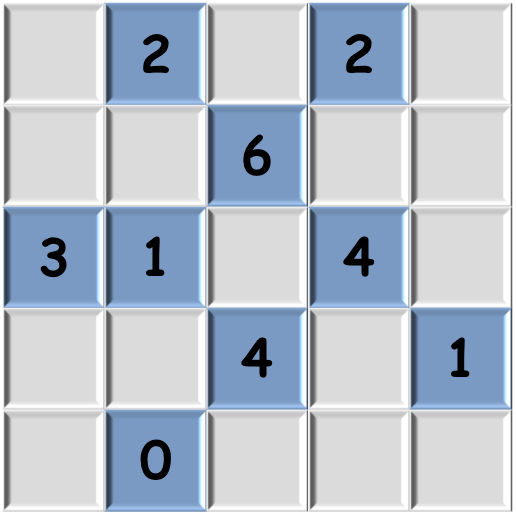
\includegraphics[width=0.3\textwidth]{figures/matrix_completion_digit.png} \qquad\qquad &   \includegraphics[width=0.47\textwidth]{figures/MC_experiment.pdf} \tabularnewline
	(a) & (b) \tabularnewline
\end{tabular}
\end{center}	
	\caption{Spectral methods for matrix recovery with missing data, where (a) is an illustration of missing data and (b) reports the empirical estimation errors of spectral methods as the sampling rate $p$ varies.  Both the relative Euclidean error $\frac{\|\widehat{\bm{M}}-\bm{M}^{\star}\|_{\mathrm{F}}}{\|\bm{M}^{\star}\|_{\mathrm{F}}}$ and the relative entrywise error $\frac{\|\widehat{\bm{M}}-\bm{M}^{\star}\|_{\infty}}{\|\bm{M}^{\star}\|_{\infty}}$ are plotted (with $\widehat{\bm{M}}$ denoting the matrix estimate and $\|\cdot\|_{\infty}$ the entrywise $\ell_{\infty}$ norm).
	\label{fig:matrix-completion-motivation}}

\end{figure}




\paragraph{Matrix recovery in the face of missing data.}

A proliferation of big-data applications has to deal with matrix estimation in the presence of missing data,  either due to the infeasibility to acquire complete observations of a massive data matrix \citep{davenport2016overview} such as the Netflix problem in recommender systems (as users only watch and rate a small fraction of movies), or because of the incentive to accelerate computation by means of sub-sampling \citep{mahoney2016lecture}.
Imagine that we are asked to estimate a large matrix $\bm{M}^{\star}=[M_{i,j}^{\star}]_{1\leq i,j\leq n}$, even though a dominant fraction of its entries are unseen.  While in general we cannot  predict anything about the missing entries,  reliable estimation might become possible if $\bm{M}^{\star}$ is known {\em a priori} to enjoy a low-rank structure, as is the case in many applications like structure from motion \citep{tomasi1992shape} and sensor network localization \citep{javanmard2013localization}. This low-rank assumption motivates the use of spectral methods.  More specifically, suppose the entries of $\bm{M}^{\star}$ are randomly sampled such that each entry  is observed independently with probability $p \in (0,1]$. An unbiased estimate $\bm{M}=[M_{i,j}]_{1\leq i,j\leq n}$ of $\bm{M}^{\star}$ can be readily obtained via  rescaling and zero filling (also called the inverse probability weighting method):
%
\begin{equation*}
	M_{i,j}=\begin{cases}
\frac{1}{p}M_{i,j}^{\star},\quad & \text{if the }(i,j)\text{-th}\text{ entry is observed},\\
0, & \text{else}.
\end{cases}
\end{equation*}
%
To capture the assumed low-rank structure of $\bm{M}^{\star}$, it is natural to resort to the best rank-$r$ approximation of $\bm{M}$ (with $r$  the true rank of $\bm{M}^{\star}$),
computable through the rank-$r$ singular value decomposition of $\bm{M}$.  Given its (trivial) success when $p=1$,  we expect the algorithm  to perform well when  $p$ is close to 1.  The key question, however, is where the algorithm stands if the vast majority of the entries is missing.
While we shall illuminate this in Chapters~\ref{chap:application-L2} and \ref{cha:Linf-theory}, Figure~\ref{fig:matrix-completion-motivation} provides some immediate numerical assessment,
which demonstrates the appealing performance of spectral methods---in terms of both Euclidean and entrywise estimation errors---even when  the missing rate is quite high.





\begin{figure}
\begin{center}
\begin{tabular}{cc}
	\includegraphics[width=0.4\textwidth]{figures/preference-score.pdf} \qquad &
	\includegraphics[width=0.4\textwidth]{figures/ranking_experiment.pdf} \tabularnewline
	(a) & (b) \tabularnewline
\end{tabular}
\end{center}	
	\caption{Spectral methods for ranking from pairwise comparisons.   (a)  illustrates the latent preference  scores $\{w_i^{\star}\}$ that govern the ranking of items. The empirical success rates in correctly identifying the top-ranked item  are plotted in (b) as $\Delta$ varies, where   $\Delta$ represents the separation between the score of the top item and that of the second-ranked item.
	\label{fig:ranking-motivation}}

\end{figure}




\paragraph{Ranking from pairwise comparisons.}
Another important application of spectral methods arises from the context of ranking,  a task  of central importance in, say, web search and recommendation systems.
In a variety of scenarios, humans find it difficult to simultaneously rank many items, but relatively easier to express pairwise preferences.
This gives rise to the problem of ranking based on pairwise comparisons.
More specifically, imagine we are given a collection of $n$ items, and wish to identify top-ranked items based on pairwise preferences (with uncertainties in comparison outcomes) between observed pairs of items.
A classical statistical model proposed by \citet{bradley1952rank, luce2012individual} postulates the existence of a set of latent positive scores $\{w_i^{\star}\}_{1\leq i\leq n}$---each associated with an item---that determines the ranks of these items.
 The outcome of the comparison between items $i$ and $j$ is generated in a way that
 %
 \begin{align*}
	 \mathbb{P}(i\text{ beats }j) = \frac{w_i^{\star}}{w_i^{\star}+w_j^{\star}}, \qquad 1\leq i,j\leq n.
\end{align*}
%
As it turns out, the preference scores  are closely related to the stationary distribution of a Markov chain associated with the above probability kernel,
thus forming the basis of spectral ranking algorithms.
To elucidate it in a little more detail, let us construct a probability transition matrix $\bm{P}^{\star}=[P_{i,j}^{\star}]_{1\leq i,j\leq n}$ with
%
\begin{align*}
	P_{i,j}^{\star}=\begin{cases}
\frac{1}{n}\cdot\frac{w_{j}^{\star}}{w_{i}^{\star}+w_{j}^{\star}}, & \text{if }i\neq j,\\
		1-\sum_{l:l\neq i}P_{i,l}^{\star}, \qquad & \text{if }i=j.
\end{cases}
\end{align*}
%
Clearly, it forms a probability transition matrix since each element is nonnegative and the entries in each row add up to one.
It is straightforward to verify that the score vector $\bm{w}^{\star}\coloneqq [w_i^{\star}]_{1\leq i\leq n}$ satisfies $\bm{w}^{\star\top} = \bm{w}^{\star\top} \bm{P}^{\star}$, namely $\bm{w}^{\star}$ is a left eigenvector of $\bm{P}^{\star}$ associated with eigenvalue one. A candidate  method then consists of (i) forming an unbiased estimate of $\bm{P}^{\star}$ (which can be easily obtained using pairwise comparison outcomes), (ii) computing its left eigenvector (in fact, the leading left eigenvector), and (iii) reporting the ranking result in accordance with the order of the elements in this eigenvector.
This spectral ranking scheme, which shares similar spirit with the celebrated {\em PageRank} algorithm \citep{page1999pagerank},
exhibits intriguing performance when identifying the top-ranked items, as showcased in the numerical experiments in Figure \ref{fig:ranking-motivation}(b).





\paragraph{A unified theme.}  In all preceding applications, the core ideas underlying the development of spectral methods can be described in a unified fashion:
%
\begin{itemize}
	\item[1.] Identify a key matrix $\bm{M}^{\star}$---which is typically unobserved---whose eigenvectors or singular vectors disclose the information being sought after;

	\item[2.] Construct a surrogate matrix $\bm{M}$ of $\bm{M}^{\star}$ using the data samples in hand, and compute the corresponding eigenvectors or singular vectors of this surrogate matrix.
\end{itemize}
%
Viewed in this light,  this monograph aims to identify key factors---e.g., certain spectral structure of $\bm{M}^{\star}$ as well as the size of the approximation error $\bm{M}-\bm{M}^{\star}$---that exert main influences on the efficacy of the resultant spectral methods.






\section{A modern statistical perspective}






The idea of spectral methods can be traced back to early statistical literature on methods of moments (e.g., \citet{pearson1894contributions,hansen1982large}),
where one seeks to extract key parameters of the probability distributions of interest by examining the empirical  moments of data.
While classical matrix perturbation theory lays a sensible foundations for the analysis of spectral methods \citep{stewart1990matrix},
the theoretical understanding can be considerably enhanced through the lens of statistical modeling---a way of thinking that has flourished in the past decade.
To the best of our knowledge, however,
a systematic and comprehensive introduction to the modern statistical foundation of spectral methods, as well as an overview of recent advances, is previously unavailable.




The current monograph aims to fill this gap by developing a coherent and accessible treatment of spectral methods from
a modern statistical perspective. Highlighting  algorithmic implications that inform practice,
our exposition gravitates around the following central questions:
how to characterize the sample efficiency of spectral methods in reaching a prescribed accuracy level,
and how to assess the stability of spectral methods in the face of random noise, missing data, and adversarial corruptions?
We underscore several distinguishing features of our treatment compared to prior studies:
%
\begin{itemize}
	\item In comparison to the worst-case performance guarantees derived solely based on classical matrix perturbation theory,
our statistical treatment emphasizes the benefit of harnessing the ``typical'' behavior of data models,
which offers key insights into how to harvest performance gains by leveraging intrinsic properties of data generating mechanisms.

	\item In contrast to classical asymptotic theory~\citep{van2000asymptotic},
		we adopt a non-asymptotic (or finite-sample) analysis framework that draws on tools from recent developments of concentration inequalities \citep{tropp2015introduction} and high-dimensional statistics \citep{wainwright2019high}. This framework accommodates the scenario where both the sample size and the number of features are enormous,
and unveils a clearer and more complete picture about the interplay and trade-off between salient model parameters.

\end{itemize}






Another unique feature of this monograph is a principled introduction of {\em fine-grained entrywise analysis} (e.g., a theory studying $\ell_{\infty}$ eigenvector perturbation),
which reflects cutting-edge research activities in this area.
This is particularly important when, for example, demonstrating the feasibility of exact clustering or perfect ranking in the aforementioned applications.
In truth, an effective entrywise analysis framework cannot be  readily obtained from classical matrix analysis alone,
and has only recently become available owing to the emergence of modern statistical toolboxes. In particular, we shall present
a powerful framework, called {\em leave-one-out analysis}, that proves effective and versatile for delivering fine-grained performance guarantees for spectral methods in a variety of problems.





\section{Organization}

We now present a high-level overview of the structure of this monograph.
%
\begin{itemize}
\item
Chapter~\ref{cha:matrix-perturbation} reviews the fundamentals of classical matrix perturbation theory for spectral analysis, focusing on $\ell_2$-type distances measured by the spectral norm and the Frobenius norm. This chapter covers the celebrated Davis-Kahan $\sin\bm{\Theta}$ theorem for eigenspace perturbation, the Wedin theorem for singular subspace perturbation, and an extension to probability transition matrices, laying the algebraic foundations for the remaining chapters.

\item
Chapter~\ref{chap:application-L2} explores the utility of $\ell_2$ matrix perturbation theory when paired with statistical tools,
presenting a unified recipe for statistical analysis empowered by non-asymptotic matrix tail bounds.
We develop spectral methods for a variety of statistical data science applications,
and derive nearly tight theoretical guarantees (up to logarithmic factors) based on this unified recipe.

\item Chapter~\ref{cha:Linf-theory} develops fine-grained perturbation theory for spectral analysis in terms of  $\ell_{\infty}$ and $\ell_{2,\infty}$ metrics, based on a leave-one-out analysis framework rooted in probability theory. Its effectiveness is demonstrated through concrete applications including community recovery and matrix completion.
  This analysis framework also enables a non-asymptotic distributional theory for spectral methods, which paves the way for uncertainty quantification in applications like noisy matrix completion. 



\item  Chapter~\ref{chapter:conclusion} concludes this monograph by identifying a few directions that are worthy of future investigation.

\end{itemize}

\noindent While this monograph pursues a coherent and accessible treatment that might appeal to a broad audience,
it does not necessarily deliver the sharpest possible results for the applications discussed herein in terms of the logarithmic terms and/or pre-constants.
The bibliographic notes at the end of each chapter contain information about the state-of-the-art theory for each application as a pointer to further readings.




\section{What is not here and complementary readings}



The topics presented in this monograph do not cover the tensor decomposition methods studied in another recent strand of work \citep{anandkumar2014tensor}.  While such tensor-based methods are also sometimes referred to as spectral methods, their primary focus is to invoke tensor decomposition to learn latent variables,  based on higher-order moments estimated from data samples.
We elect not to discuss this class of methods but instead refer the interested reader to the recently published monograph by \citet{MAL-057}.
Another monograph by \citet{kannan2009spectral} provides an in-depth computational and algorithmic treatment of spectral methods from the perspective of theoretical computer science.
The applications and results covered therein (e.g., fast matrix multiplication)  complement the ones presented in the current monograph.
In addition, spectral methods have been frequently employed to initialize nonconvex optimization algorithms. We will not elaborate on the nonconvex optimization aspect here but instead recommend the reader to the recent overview article by \citet{chi2019nonconvex}.  Finally, spectral methods are widely adopted to estimate high-dimensional covariance and precision matrices, and extract latent factors for econometric and statistical modeling. This topic alone has a huge literature, and we refer the interested reader to \citet{fan2020statistical} for in-depth discussions.





\section{Notation}

Before moving forward, let us introduce some notation that will be used throughout this monograph.


First of all, we reserve boldfaced symbols  for vectors, matrices and tensors.
For any matrix $\bm{A}$, let $\sigma_{j}(\bm{A})$ (resp.~$\lambda_{j}(\bm{A})$) represent its $j$-th largest singular value (resp.~eigenvalue).
In particular, $\sigma_{\max}(\bm{A})$ (resp.~$\lambda_{\max}(\bm{A})$) stands for the largest singular value (resp.~eigenvalue) of $\bm{A}$,
while $\sigma_{\min}(\bm{A})$ (resp.~$\lambda_{\min}(\bm{A})$) indicates the smallest singular value (resp.~eigenvalue) of $\bm{A}$.
We use $\bm{A}^{\top}$ to denote the transpose of $\bm{A}$, and
let $\bm{A}_{i,\cdot}$ and $\bm{A}_{\cdot,i}$ indicate the $i$-th row and the $i$-th column of $\bm{A}$, respectively.
We follow standard conventions by letting
$\bm{I}_{n}$ be the $n\times n$ identity matrix, $\bm{1}_{n}$ the $n$-dimensional all-one vector, and $\bm{0}_{n}$ the $n$-dimensional all-zero vector;
we shall often suppress the subscript as long as it is clear from the context.
The $i$-th standard basis vector is denoted by $\bm{e}_i$ throughout.
The notation $\mathcal{O}^{n\times r}$ ($r\leq n$) represents the set of all $n\times r$ orthonormal matrices (whose columns are orthonormal). Moreover, we refer to $[n]$ as the set $\{1,\cdots, n\}$.


Next, we  turn to vector and matrix norms. For any vector $\bm{v}$, we denote by $\|\bm{v}\|_2$, $\|\bm{v}\|_1$ and $\|\bm{v}\|_{\infty}$  its $\ell_2$ norm, $\ell_1$ norm and $\ell_{\infty}$ norm, respectively.
 For any matrix $\bm{A}=[A_{i,j}]_{1\leq i\leq m,1\leq j\leq n}$,  we let $\|\bm{A}\|$, $\|\bm{A}\|_{*}$, $\|\bm{A}\|_{\mathrm{F}}$ and $\|\bm{A}\|_{\infty}$  represent respectively its spectral norm (i.e., the largest singular value of $\bm{A}$), its nuclear norm (i.e., the sum of singular values of $\bm{A}$), its Frobenius norm (i.e., $\|\bm{A}\|_{\mathrm{F}} \coloneqq \sqrt{\sum_{i,j}A_{i,j}^2}$), and its entrywise $\ell_{\infty}$ norm (i.e., $\|\bm{A}\|_{\infty} \coloneqq \max_{i,j}|A_{i,j}|$).
We also refer to $\|\bm{A}\|_{2,\infty}$  as the $\ell_{2,\infty}$ norm  of $\bm{A}$,
defined as $\|\bm{A}\|_{2,\infty} \coloneqq \max_i \|\bm{A}_{i,\cdot}\|_2$.
Similarly, we define the $\ell_{\infty,2}$ norm  of $\bm{A}$ as $\|\bm{A}\|_{\infty,2} \coloneqq \|\bm{A}^{\top}\|_{2,\infty}$.
In addition, for any matrices $\bm{A}=[A_{i,j}]_{1\leq i\leq m,1\leq j\leq n}$ and $\bm{B}=[B_{i,j}]_{1\leq i\leq m,1\leq j\leq n}$,
the inner product of $\bm{A}$ and $\bm{B}$ is defined as and denoted by $\langle \bm{A}, \bm{B} \rangle = \sum_{1\leq i\leq m,1\leq j\leq n} A_{i,j} B_{i,j} = \mathsf{Tr}(\bm{A}^{\top}\bm{B})$. 


When it comes to diagonal matrices,
 we employ $\mathsf{diag}([\theta_1, \theta_2, \cdots, \theta_r])$ to abbreviate the diagonal matrix with diagonal elements $\theta_1, \cdots, \theta_r$.
For any diagonal matrix $\bm{\Theta} = \mathsf{diag}([\theta_1, \theta_2, \cdots, \theta_r])$,
we adopt the shorthand notation $\sin \bm{\Theta} \coloneqq \mathsf{diag}([\sin\theta_1, \sin\theta_2, \cdots, \sin\theta_r])$; the notation $\sin^2\bm{\Theta}$, $\cos\bm{\Theta}$, and $\cos^2\bm{\Theta}$ is defined analogously.







Finally, this monograph makes heavy use of the following standard notation:
(1) $f(n)=O\left(g(n)\right)$ or
$f(n)\lesssim g(n)$ means that there exists a universal constant $c>0$ such
that $\left|f(n)\right|\leq c|g(n)|$ holds for all sufficiently large $n$; (2) $f(n)\gtrsim g(n)$ means that there exists a universal constant $c>0$ such
that $|f(n)|\geq c\left|g(n)\right|$ holds for all sufficiently large $n$;
 (3) $f(n)\asymp g(n)$ means that there exist universal constants $c_{1},c_{2}>0$
such that $c_{1}|g(n)|\leq|f(n)|\leq c_{2}|g(n)|$ holds for all sufficiently large $n$;
and (4) $f(n)=o(g(n))$ indicates that $f(n)/g(n)\rightarrow 0$ as $n\rightarrow \infty$.
Additionally, we sometimes use $f(n)\gg g(n)$ (resp.~$f(n)\ll g(n)$) to indicate that there exists some sufficiently large (resp.~small) universal constant $c >0$ such that $|f(n)|\geq c \left|g(n)\right|$ (resp.~$|f(n)|\leq c \left|g(n)\right|$).




